\documentclass{article}
\usepackage[utf8]{inputenc}
\usepackage[spanish]{babel}
\usepackage{amsmath}
\usepackage{amssymb}
\usepackage{amsfonts}
\usepackage{hyperref}
\usepackage{cite}
\usepackage{textcomp}
\usepackage{graphicx}
\usepackage{pgfplots}
\usepackage{geometry}
\usepackage{booktabs}
\hypersetup{
    colorlinks=true,
    linkcolor=black,
    citecolor=green,
    filecolor=magenta,      
    urlcolor=cyan,
}
\geometry{
  top=3cm,
  bottom=3cm,
  left=3cm,
  right=3cm
}

\title{Estadística 1}
\author{Jorge Miguel Alvarado Reyes}
\date{16 Agosto 2023}

\setlength{\parindent}{0pt}
\begin{document}

\begin{titlepage}
    \begin{center}
        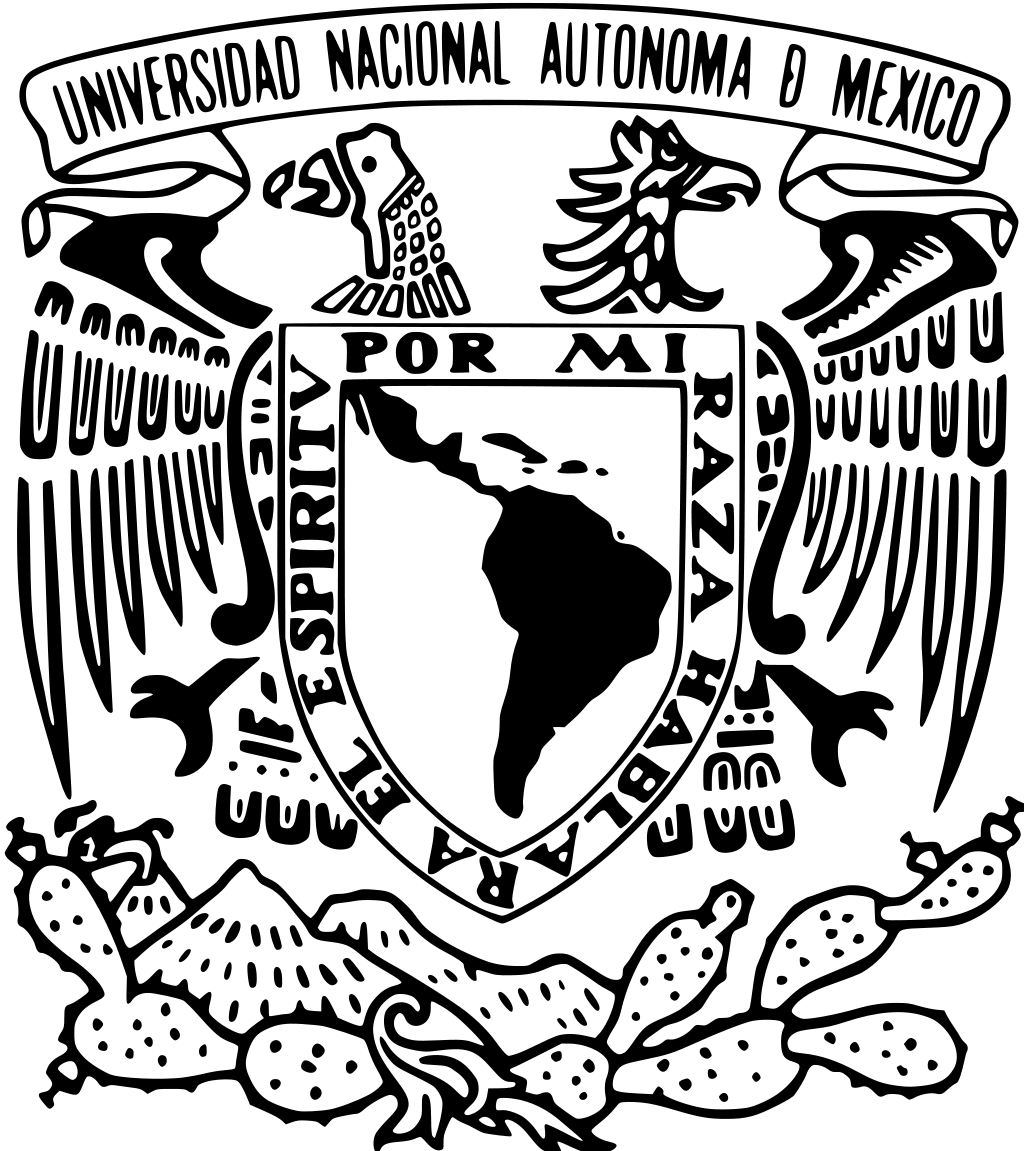
\includegraphics[width=0.2\textwidth]{../../unam.png}
        \vspace*{.5cm}

        \LARGE
        \textbf{Universidad Nacional Autónoma de México}

        \vspace{0.5cm}
        \LARGE
        Facultad de Estudios Superiores Acatlán

        \vspace{2cm}

        \textbf{Apuntes} \\
        Investigación sobre pruebas de normalidad

        \vfill

        \vspace{1cm}

        \textbf{\large Autor:} \\
        Jorge Miguel Alvarado Reyes \\
        \vspace{.5cm}
        \normalsize \today

    \end{center}
\end{titlepage}
\newpage

\tableofcontents

\newpage

\section{Introducción}

La pruebas de normalidad sirven para determinar si los datos de una muestra siguen una distribución normal, Esta distribución es fundamental en estadística debido a que muchos análisis estadísticos asumen que los datos se distribuyen normalmente. Si los datos no cumplen con esta suposición, los resultados de dichos análisis podrían ser engañosos.

\section{Prueba de Lilliefors}

La Prueba de Lilliefors es una modificación de la prueba de Kolmogorov-Smirnov, diseñada específicamente para evaluar la normalidad de una muestra cuando los parámetros de la distribución normal (media y varianza) no son conocidos de antemano. A diferencia de la prueba de Kolmogorov-Smirnov, que requiere que la media y la varianza de la población sean conocidas, la Prueba de Lilliefors estima estos parámetros directamente de los datos de la muestra.

La hipótesis nula se rechaza si la estadística de prueba calculada excede un valor crítico, lo cual indica una discrepancia significativa entre la distribución de la muestra y una distribución normal teórica. La estadística de prueba se basa en la máxima diferencia absoluta entre la función de distribución empírica de la muestra y la función de distribución acumulativa normal ajustada, como se muestra en la fórmula siguiente:

\[
    D = \max | F_n(x) - F(x; \hat{\mu}, \hat{\sigma}) |
\]

donde:
\begin{itemize}
    \item \(D\) es la máxima diferencia absoluta entre la función de distribución empírica \(F_n(x)\) y la función de distribución acumulativa normal \(F(x; \hat{\mu}, \hat{\sigma})\).
    \item \(F_n(x)\) representa la función de distribución empírica basada en los datos de la muestra.
    \item \(F(x; \hat{\mu}, \hat{\sigma})\) es la función de distribución acumulativa normal teórica, con la media \(\hat{\mu}\) y la varianza \(\hat{\sigma}\) estimadas a partir de los datos de la muestra.
\end{itemize}

Para llevar a cabo la Prueba de Lilliefors en el entorno de R, se puede utilizar el comando \texttt{lillie.test} del paquete \texttt{nortest}.


\section{Prueba de Cramér-van Mises}

La Prueba de Cramér-van Mises es un método estadístico utilizado para evaluar la hipótesis de que una muestra dada se distribuye de acuerdo con una distribución teórica específica. A diferencia de otras pruebas de bondad de ajuste, esta prueba considera la diferencia cuadrada entre la función de distribución acumulada empírica de la muestra y la teórica, integrada a lo largo de todo el rango de los datos. Es especialmente útil para análisis en los que se requiere una estimación de distancia mínima y puede aplicarse en dos contextos principales: una muestra y dos muestras.

\subsection*{Una Muestra}

Para una muestra, la estadística de prueba se calcula mediante la fórmula:

\[
    T = nw^2 = \frac{1}{12n} + \sum_{i=1}^{n}\left[\frac{2i - 1}{2n} - F(x_i)\right]^2
\]

donde \(F\) es la función de distribución acumulada teórica y \(x_i\) son los valores observados, ordenados de manera creciente. Si el valor calculado de \(T\) excede el valor crítico tabulado, se rechaza la hipótesis nula de que los datos siguen la distribución \(F\).

\subsection*{Dos Muestras}

En el contexto de dos muestras, la prueba compara las distribuciones empíricas de dos conjuntos de datos para evaluar si provienen de la misma distribución subyacente. La estadística de prueba para dos muestras se calcula como:

\[
    U^2 = \frac{n m}{n + m} \int_{-\infty}^{\infty} [F_n(x) - G_m(x)]^2 dH(x)
\]

donde:
\begin{itemize}
    \item \(n\) y \(m\) son los tamaños de las dos muestras.
    \item \(F_n(x)\) es la función de distribución acumulada empírica de la primera muestra.
    \item \(G_m(x)\) es la función de distribución acumulada empírica de la segunda muestra.
    \item \(H(x)\) es la función de distribución acumulada empírica combinada de ambas muestras.
    \item La integración se realiza a lo largo de todo el rango de los datos.
\end{itemize}

Un valor grande de \(U^2\) indica una evidencia significativa contra la hipótesis nula de que las dos muestras provienen de la misma distribución subyacente.


\section{Prueba de Shapiro-Wilk}

Sirve para determinar si un conjunto de datos se distribuye normalmente, fue publicada en 1965 por Samuel Shapiro y Martin Wilk, esta prueba es considerada como una de las más potentes para el contraste de normalidad.

La hipótesis nula ($H_0$) plantea que la muestra proviene de una población normalmente distribuida. El estadístico de prueba W se calcula a partir de los datos de la muestra, utilizando una fórmula específica que involucra los valores ordenados de la muestra, la media muestral y ciertas constantes $a_i$, que se derivan de las covarianzas, varianzas y medias de una muestra normalmente distribuida. La prueba tiene un rango para $W$ de 0 a 1, y la hipótesis nula se rechaza si W es demasiado pequeño, indicando que la distribución de los datos no es normal

\[W = \frac{\left(\sum_{i=1}^{n}a_{i}x_{(i)}\right)^{2}}{\sum_{i=1}^{n}(x_{i}-\overline{x})^{2}}
\]

Aunque la prueba de Shapiro-Wilk es altamente eficaz, tiene limitaciones, especialmente en muestras muy grandes, donde puede ser demasiado sensible a desviaciones insignificantes de la normalidad. Por esta razón, es importante considerar el contexto y el tamaño de la muestra al interpretar los resultados.

En R se puede realizar la prueba con la función \texttt{shapiro.test}.

\section{Prueba de Anderson-Darling}

La prueba de Anderson-Darling es un método estadístico utilizado para evaluar si un conjunto de datos sigue una distribución específica. Aunque se aplica comúnmente para verificar la normalidad de los datos, la prueba puede utilizarse para otras distribuciones como la exponencial, la Weibull, entre otras.

El núcleo de esta prueba radica en dos hipótesis fundamentales:

\begin{itemize}
    \item Hipótesis nula (\(H_0\)): Los datos se ajustan a la distribución específica.
    \item Hipótesis alternativa (\(H_1\)): Los datos no se ajustan a la distribución específica.
\end{itemize}

El estadístico de prueba se calcula de la siguiente manera, donde la fórmula ajusta el enfoque según la distribución de interés.
\[A^2 = -n - \frac{1}{n} \sum_{i=1}^{n} (2i-1) \left[ \ln(F(x_i)) + \ln(1-F(x_{n+1-i})) \right]\]

Donde:
\begin{itemize}
    \item \(A^2\): Es el estadístico de prueba Anderson-Darling, que se utiliza para evaluar si una muestra de datos proviene de una población con una distribución específica.
    \item \(n\): Es el tamaño de la muestra, es decir, el número total de observaciones en la muestra.
    \item \(x_i\): Son los datos ordenados de menor a mayor. \(x_1\) sería el dato más pequeño, y \(x_n\) el dato más grande.
    \item \(F(x_i)\): Es la función de distribución acumulada teórica evaluada en \(x_i\). Esta función representa la probabilidad de que una variable aleatoria sea menor o igual que \(x_i\).
    \item \(2i-1\): Es un factor que se multiplica por el logaritmo de las funciones de distribución, ajustando la ponderación de cada término en la suma.
\end{itemize}

La interpretación de los resultados de la prueba de Anderson-Darling se basa en el valor \(p\) obtenido: un valor \(p\) bajo sugiere el rechazo de la hipótesis nula, indicando que los datos no se ajustan a la distribución especificada.

\section{Prueba de Jarque-Bera}

La prueba de Jarque-Bera es una herramienta estadística de bondad de ajuste que evalúa si una muestra de datos tiene las características de asimetría y curtosis que se esperarían de una distribución normal. Desarrollada por Carlos Jarque y Anil K. Bera, esta prueba es especialmente valiosa para analizar grandes muestras de datos. A diferencia de otras pruebas de normalidad, como la prueba de Shapiro-Wilk, que pueden perder precisión con tamaños de muestra muy grandes (por ejemplo, más de 2000 observaciones), la prueba de Jarque-Bera mantiene su fiabilidad incluso en estos casos.

La prueba de Jarque-Bera se basa en la comparación de la asimetría y curtosis de los datos de la muestra con los valores esperados en una distribución normal (asimetría de cero y curtosis de tres), lo cual indica una distribución perfectamente simétrica alrededor de la media. La estadística de prueba de Jarque-Bera se calcula como sigue:

\[JB = \frac{n}{6} \left(S^2 + \frac{1}{4}(K - 3)^2\right)\]

Donde:
\begin{itemize}
    \item \(JB\): Es la estadística de prueba Jarque-Bera, utilizada para evaluar la normalidad de los datos basándose en asimetría y curtosis.
    \item \(n\): Es el número de observaciones en la muestra.
    \item \(S\): Es la asimetría de la muestra. La asimetría mide la falta de simetría en la distribución de los datos, con un valor de cero indicando simetría perfecta.
    \item \(K\): Es la curtosis de la muestra. La curtosis mide la "colinealidad" de los datos, con un valor de tres indicando una curtosis normal (distribución mesocúrtica).
    \item La hipótesis nula (H0): Se asume que los datos siguen una distribución normal, es decir, que la asimetría es cero y la curtosis es tres.
    \item La hipótesis alternativa (H1): Se asume que los datos no siguen una distribución normal, indicado por una asimetría y/o curtosis que difiere significativamente de los valores esperados en una distribución normal.
\end{itemize}


Para llevar a cabo la prueba de Jarque-Bera en R, se pueden utilizar paquetes como \texttt{tseries} con la función \texttt{jarque.bera.test}, o el paquete \texttt{moments} con la función \texttt{jarque.test}.

\section{Conclusiones}

Las pruebas de normalidad como la Prueba de Lilliefors, Prueba de Cramér-van Mises, Prueba de Shapiro-Wilk, Prueba de Anderson-Darling, y Prueba de Jarque-Bera, ofrecen herramientas valiosas para evaluar la adecuación de los datos a la distribución normal. Cada prueba tiene sus propias fortalezas y limitaciones, y la elección de la prueba adecuada puede depender del tamaño de la muestra y los objetivos específicos del análisis. Utilizar múltiples pruebas de normalidad puede proporcionar una visión más completa de la distribución de los datos y ayudar a la toma de desiciones.

\newpage

\section{Referencias}

\begin{enumerate}
    \item Benites, L. (2021, diciembre 19). Prueba de Lilliefors para normalidad y distribuciones exponenciales. Statologos. \url{https://statologos.com/prueba-de-lillie-fors/}
    \item Cramér-von Mises test. (s/f). Encyclopediaofmath.org. Recuperado el 24 de febrero de 2024, de \url{https://encyclopediaofmath.org/wiki/Cram%C3%A9r-von_Mises_test}
    \item Moler, M. [@madelenemoler7057]. (2019, noviembre 13). ¿QUÉ ES UNA PRUEBA DE NORMALIDAD? - Estadística aplicada a la Investigación Científica. Youtube. \url{https://www.youtube.com/watch?v=LoCR_D4D4uc}
    \item Parrales, H. (2023, diciembre 10). Pruebas de Normalidad. Aprobados. \url{https://aprobados.net/pruebas-de-normalidad/}
    \item Prueba de normalidad. (s/f). Datatab.es. Recuperado el 24 de febrero de 2024, de \url{https://datatab.es/tutorial/test-of-normality}
    \item Wikipedia contributors. (s/f-a). Criterio de Cramér-von Mises. Wikipedia, The Free Encyclopedia. \url{https://es.wikipedia.org/w/index.php?title=Criterio_de_Cram%C3%A9r-von_Mises&oldid=144368388}
    \item Wikipedia contributors. (s/f-b). Prueba de Anderson-Darling. Wikipedia, The Free Encyclopedia. \url{https://es.wikipedia.org/w/index.php?title=Prueba_de_Anderson-Darling&oldid=148231894}
    \item Wikipedia contributors. (s/f-c). Prueba de Lilliefors. Wikipedia, The Free Encyclopedia. \url{https://es.wikipedia.org/w/index.php?title=Prueba_de_Lilliefors&oldid=147771725}
\end{enumerate}



\end{document}